\documentclass{article}
\usepackage{multicol}
\usepackage{fullpage}
\usepackage[english]{babel}
\usepackage{blindtext}
\usepackage{url}
\usepackage[round]{natbib}
\usepackage{Sweave}
\usepackage{graphicx}
\addtolength{\oddsidemargin}{-0.4in}
\addtolength{\evensidemargin}{-0.3in}
\addtolength{\textwidth}{0.7in}
\addtolength{\topmargin}{-0.4in}
\addtolength{\textheight}{0.8in}
\begin{document}
\title {pheno2geno}
\author{
Konrad Zych\,$^{1,2}$, 
Danny Arends\,$^{2,}$,
 Ritsert C. Jansen\,$^{2}$
}
\maketitle
{\noindent}1. Faculty of Biochemistry, Biophysics and Biotechnology, Jagiellonian University in Krakow, Poland \\*
2. Groningen Bioinformatics Center, University of Groningen, The Netherlands

\newpage
\section{General introduction}

{\noindent}Genetical Genomics \citep{Jansen:2001388} is powerful method, providing world of life sciences with tool to look deep inside the complex relation between genetic information stored by DNA and final outcome of its processing - phenotype. And because this is the core dogma of modern biology, every method helping us to understand it better is of high importance to scientific world. 

{\noindent}Great power often comes for high price, though. To perform GG studies one has to obtain both phenotypic and genotypic data, that are subsequently being matched. This not only elevates costs of experiment, but also introduces number of human errors, e.g. mismatching/mislabeling of arrays.

{\noindent}This brought us back to DNA to phenotype dogma. And we came up with idea of creating genetic map out of gene expression data. This means the same power for less then half of the cost and effort. Procedure is easy enough to be conducted by inexperienced R user and for advanced users we offer variety of extra functionalities to make their analysis fit their needs.
\subsection{R programming language}
R programming language is powerful, yet easy-to-use. There is graphical interface available for Windows, Mac OS and Linux. Every package/function comes with easily accessible help file and, most importantly, R provides user with handfuls of statistical functionalities. To start your adventure with R just go to: http://cran.r-project.org/, select your operating system, install it, and you're ready to enter the world of R.
\subsection{Downloading and installing package}
R packages contribute to power of this language more than anything. Using then, you can extend basic R to powerful tool perfectly suited to your personal needs. Installing package is really easy, just open R gui and type:
> install me
> or what?
or use Packages menu (just click on Install Packages, select a mirror and than select package pheno2geno).

\newpage
\section{Data}

\subsection{Data files' structure}
{\noindent}In order to ensure smooth work of our package, we specified strict rules about data files provided. If below mentioned requirements are met and filenames are default, user don't have to provide reading function with any parameters. If your more advanced R user, your data files are of different format or you have data already inside R environment, please see section 4.1. 
\subsubsection{Phenotype data for offspring}
This data is crucial and analysis cannot be run without it. Default filename is offspring\_phenotypes.txt. Rows correspond to markers and columns to individuals. File should contain only numeric values apart from first row, containing unique column names and first column containing unique row names. Rows and columns with non-numeric values are removed. All values should be separated by tabs. In normal practice first row has one element less then others (no column name for column containing rownames).
\subsubsection{Phenotype data for founders}
This data is optional but really important for the analysis, so we recommend to provide it. Default filename is founders\_phenotypes.txt. Data structure inside the file should be the same as in offspring phenotype file. Also row names should match, because non-matching rows are removed.
\subsubsection{Genotype data for offspring}
This data is optional and doesn't have any impact on analysis, could be only used for creating cross object out of existing data using our software. Default filename is offspring\_genotypes.txt. Genotypes should be coded as 0,1 and NA. Data structure inside the file should be the same as in offspring and founders phenotype files. Row names should match, because non-matching rows are removed. 
\subsubsection{Genetic map}
This data is optional and could be used for comparison with map created by our software or for ordering markers in output cross. Default filename is maps\_genetic.txt. File should contain three columns - marker name, chromosome number and position on chromosome in cM. Second and third column should contain numeric values without NAs, NaNs, etc. First column should contain unique marker names, matching ones in phenotype files.
\subsubsection{Physical map}
Exactly the same as in genetic map, but position on chromosome should be in Mbp.

\newpage
\section{Basic workflow}
\subsection{Loading data into workflow}
\subsubsection{readFiles function}
If data is formatted as specified in chapter 2 and files are having default names, you just have to type: 
\begin{Schunk}
\begin{Sinput}
> population <- readFiles(founders_groups = c(0, 0, 1, 1))
\end{Sinput}
\end{Schunk}
 into Rgui (make sure your working directory is the one containing data files) and it's all done. Parameter founders\_groups specifies in which column of parental file which parent is. Eg. you measured gene expression of both parents twice. Results for one of those are in first two columns, for the other - in following two. Then your function call will look exactly like one given above. 
If you don't like words founders, offspring and map and would like to use more friendly parents, children and treasure\_map instead, just type:
\begin{Schunk}
\begin{Sinput}
> population <- readFiles(offspring = "children", founders = "parents", 
+     map = "treasure_map", founders_groups = c(0, 0, 1, 1))
\end{Sinput}
\end{Schunk}
{\noindent}Function will then look for eg genetic map in file treasure\_map\_genetic.txt.For more info about the function type in R:
\begin{Schunk}
\begin{Sinput}
> `?`(createPopulation)
\end{Sinput}
\end{Schunk}
\subsubsection{createPopulation function}
Loading data from files is not always the best idea. Imagine you loaded your data into R already, for example to normalize it. Saving it back to disk and reading again into R means wasting your time. In this case you can use createPopulation function:
\begin{Schunk}
\begin{Sinput}
> population <- createPopulation(offspring_phenotypes, founders, 
+     founders_groups, offspring_genotypes, maps_genetic, maps_physical)
\end{Sinput}
\end{Schunk}
just listing objects that contain phenotype, genotype data and maps. For example if you have phenotype matrix called phenotypes for both founders(columns 1-4) and offspring(5-100) you can load that into population object using:
\begin{Schunk}
\begin{Sinput}
> population <- createPopulation(phenotypes[, 1:4], phenotypes[, 
+     5:100], c(0, 0, 1, 1))
\end{Sinput}
\end{Schunk}
{\noindent}For more info about the function type in R:
\begin{Schunk}
\begin{Sinput}
> `?`(createPopulation)
\end{Sinput}
\end{Schunk}
\subsubsection{faking population object}
Sometimes you nede pretty simple and small dataset to do samoe testing on. Or to be able to play with, to learn how to use the package. Like in this manual. In this step fakePopulation function comes handy: 
\begin{Schunk}
\begin{Sinput}
> population <- fakePopulation()
\end{Sinput}
\end{Schunk}
{\noindent}There is a lot of parameters you can provide to this function to get more sophisticated datasets, but for our use default one (founders measured twice, 250 offspring individuals, 1000 markers spread evenly over 10 chromosomes, 
RIL population obtained using selfing) will be perfect. For more info about the function type in R:
\begin{Schunk}
\begin{Sinput}
> `?`(fakePopulation)
\end{Sinput}
\end{Schunk}
\newpage
\subsection{Inspecting data}
\subsubsection{Founders data}
We provide you we function to plot founders data for brief inspection. Let's inspect first 20 markers of just faked population object:

\begin{Schunk}
\begin{Sinput}
> plotParentalExpression(population, 1:20)
\end{Sinput}
\end{Schunk}
\includegraphics{manual-009}

{\noindent}Empty circles (blue for parent "0" and red for parent "1") on the plot show gene expression values, green lines - mean values for each marker.
\newpage
\subsubsection{Offspring data}
We can also inspect gene expression values for offspring. To show plot for first 20 markers:
\begin{Schunk}
\begin{Sinput}
> plotChildrenExpression(population, 1:20)
\end{Sinput}
\end{Schunk}
\includegraphics{manual-010}

{\noindent}Boxplot (in black) shows gene expression values for offspring. On those, founders data is overlayed, depicted as in plotParentalExpression.
\newpage
\subsubsection{Single markers distribution}
This kind of plot gives possibility to make sure that our data is distributed as we supposed. In our case, RIL with selfing, we expect in all markers mixture of two normal distributions.
In our example we will look at values for third marker:
\begin{Schunk}
\begin{Sinput}
> plotMarkerDistribution(population, 3, 2)
\end{Sinput}
\end{Schunk}
\includegraphics{manual-011}

{\noindent}First parameter is object of class population, then number or name of marker to be shown and number of normal distributions to be fitted (more than 1).
\newpage
\subsection{Rank product analysis}
RankProd \citep{Hong:2006} is a R package using Rank Product \citep{Breitling200483} method to detect genes showing differential expression, especially in microarray experiments. As so, it fits our needs perfectly and that's why it's incorporated into our workflow. 
In majority of cases object of class population is the only parameter while calling findDiffExpressed function. RP, main function of RankProd, is always verbose, so exptect something like:
\begin{Schunk}
\begin{Sinput}
> population <- findDiffExpressed(population)
\end{Sinput}
\begin{Soutput}
Rank Product analysis for two-class case 
 
Starting 100 permutations... 
Computing pfp .. 
Outputing the results .. 
\end{Soutput}
\end{Schunk}

{\noindent}If you're more experienced user and would like to provide RP function with additional parameters, it's possible. Just provide preprocessData funtion with them and they will be send directly to RP function. For further information see help file of RP.

\subsection{toGenotypes function - introduction}
After RankProduct analysis is done, it's time for magic to happen,  very essence of this package - creating genetic map out of gene expression data. Because this function call is much more complicated than any other in the 
package, we summarized most important parameters in table below:

 \begin{tabular}{ | c | p{5.5cm} | p{4.5cm}| }
  \hline                       
  parameter name & description & possible values \\ \hline
  treshold & treshold p-value to classify gene as differentially expressed & 0-1 \\ \hline
  overlapInd & how many individuals may overlap between distributions & 0-nr of individuals  \\ \hline
  proportion & specifying how many normal distributions are expected and percentage of individuals in every group  & vector of 0-100 summing up to 100  \\ \hline
  margin & proportion is allowed to varry between this margin (2 sided)  & 0-min(proportion) \\ \hline
\end{tabular}

{\noindent}and we strongly recommend to see help file of this function:
\begin{Schunk}
\begin{Sinput}
> `?`(toGenotypes)
\end{Sinput}
\end{Schunk}

\subsection{Example function call for RILs}
In data from RIL population (like one we faked in section 3.1.3), we expect two normal distributions in gene expression data. Each group should contain 50 percent of individuals. Proportion parameter should then have value c(50,50).
This is default one. We would like to save genotype data created by toGenotypes and order it using genetic map. In this case for all the parameters we use default values.  Function call then should look like:
\begin{Schunk}
\begin{Sinput}
> cross <- toGenotypes(population)
\end{Sinput}
\end{Schunk}

{\noindent}After function is executed, our data is stored inside (a bit enhanced) cross object. We can use R/qtl functions to plot it. Most informative plots will be:

{\noindent}- plot.rf - showing recombination factors between markers
\begin{Schunk}
\begin{Sinput}
> plot.rf(cross)
\end{Sinput}
\end{Schunk}
\includegraphics{manual-015}
\newpage
{\noindent}- plot.map - showing how markers are spread on the chromosomes
\begin{Schunk}
\begin{Sinput}
> plot.map(cross)
\end{Sinput}
\end{Schunk}
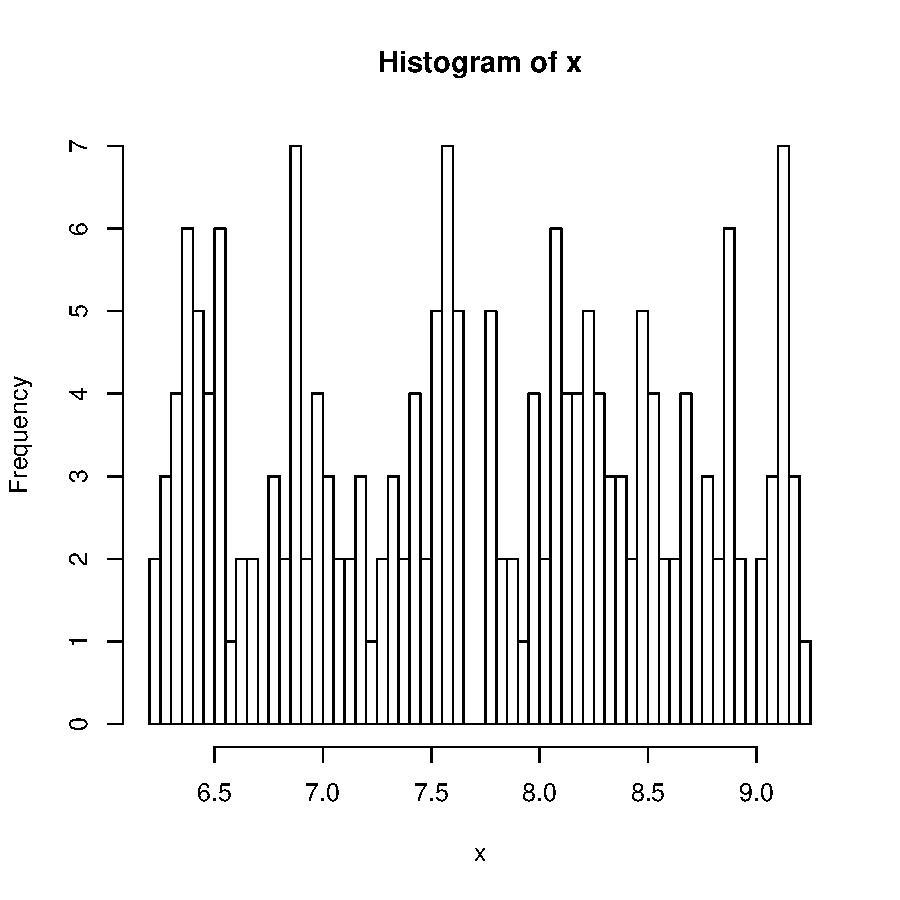
\includegraphics{manual-016}
\newpage
{\noindent}- geno.image showing our newly created genotypes
\begin{Schunk}
\begin{Sinput}
> geno.image(cross)
\end{Sinput}
\end{Schunk}
\includegraphics{manual-017}
\newpage
\subsection{Example workflow for BC}


	
	plot.rf(cross, main="bc toGenotypes example")

{\noindent}We start with faking population object with data for Back Cross:
\begin{Schunk}
\begin{Sinput}
> population <- fakePopulation(type = "bc")
\end{Sinput}
\end{Schunk}

{\noindent}The only, but very important difference lays in distribution of the data. We can inspect it using plotMarkerDistribution:
\begin{Schunk}
\begin{Sinput}
> plotMarkerDistribution(population, 3, 2)
\end{Sinput}
\end{Schunk}

{\noindent}Next step, Rank Product analysis, is exactly the same as for RILs:
\begin{Schunk}
\begin{Sinput}
> population <- findDiffExpressed(population)
\end{Sinput}
\end{Schunk}

\newpage
{\noindent}After checking distribution of the data (obviously checking distribution of one marker is not enough, but that step is just for visual inspection, toGenotypes is
checking distribution of markers automatically) and finding differentially expressed genes, we can use toGenotypes function:
\begin{Schunk}
\begin{Sinput}
> cross <- toGenotypes(population, genotype = "simulated", proportion = c(25, 
+     75), orderUsing = "map_genetic", treshold = 0.1)
\end{Sinput}
\end{Schunk}

{\noindent}And plot recombination factors between individuals:
\begin{Schunk}
\begin{Sinput}
> plot.rf(cross, main = "BC workflow example")
\end{Sinput}
\end{Schunk}

\newpage
\subsection{Example workflow for F2 cross}
{\noindent}Again we start with faking population object. This time with data for F2 cross:
\begin{Schunk}
\begin{Sinput}
> population <- fakePopulation(type = "f2")
\end{Sinput}
\end{Schunk}

{\noindent}This time we expect totally different distribution of data. Mixture of three normal distributions with proportions 25/50/25:
\begin{Schunk}
\begin{Sinput}
> plotMarkerDistribution(population, 3, 3)
\end{Sinput}
\end{Schunk}

{\noindent}Finding differentially expressed genes we still do the same:
\begin{Schunk}
\begin{Sinput}
> population <- findDiffExpressed(population)
\end{Sinput}
\end{Schunk}

\newpage
{\noindent}Finally, we can use toGenotypes function:
\begin{Schunk}
\begin{Sinput}
> cross <- toGenotypes(population, genotype = "simulated", proportion = c(25, 
+     50, 25), orderUsing = "map_genetic", treshold = 0.1)
\end{Sinput}
\end{Schunk}

{\noindent}And plot recombination factors between individuals:
\begin{Schunk}
\begin{Sinput}
> plot.rf(cross, main = "f2 toGenotypes example")
\end{Sinput}
\end{Schunk}

\newpage
\section{Postprocessing of cross object}

\subsection{Comparing created map to }
\blindtext
\subsection{Rank product analysis}
\blindtext
\subsection{Uncommon types of crosses}
\blindtext
\subsection{Modifying splitting options}
\blindtext
\subsection{Filtering markers}
\blindtext
\subsection{Cross object}
\blindtext
\subsubsection{Forming linkage groups and \\* ordering markers}
\blindtext
\subsubsection{Post-processing of cross object}
\blindtext

\newpage
\section{Built-in plotting routines}
\subsection{plotChildrenExpression}
\blindtext[2]
\subsection{plotParentalExpression}
\blindtext[2]
\subsection{plotMapComparison}
\blindtext[2]
\subsection{plotMarkerDistribution}
\blindtext[2]
\newpage
\section{Big datasets}

\subsection{Problematic handling of big data by R}
\blindtext
\subsection{C preprocessing}
\blindtext
\subsection{Other solutions}
\blindtext

\newpage
\section{Package development \& collaboration}
\newpage
\section{References}
\bibliographystyle{plainnat}
\bibliography{manual}
\end{document}
